\section{Ablauf des Hauptprogramms} \label{hauptprogrammKapitel}
Um die Fahrzeugsteuerung zu starten, muss die Datei \textit{main.php} ausgeführt werden. Obligatorisch für die Fahrzeugsteuerung ist die Abschnittsüberwachung (\textit{abschnittueberwachung.php}), welche vor dem Start der Fahrzeugsteuerung ausgeführt werden muss. Auf die genaue Verwendung der Abschnittsüberwachung wird in Kapitel \ref{main_5} eingegangen. In der folgenden Abbildung \ref{fig:hauptprogramm} ist der schematische Ablauf des Hauptprogramms abgebildet, welcher auch grob dem Aufbau dieses Kapitel dient.
\begin{center}
\begin{figure}
\centering
\begin{tikzpicture}[node distance=1cm, auto,]
\node[punkt] (a) {Einbindung aller benötigten Dateien};
\node[below=of a, punkt] (b) {Einlesen von statischen und mehrfach verwendeter Daten aus der \textit{SQL}-Datenbank in den Cache};
\node[below=of b, punkt](c) {Ermittlung aller Fahrzeuge im eingleisigen Netz und den zugehörigen Daten};
\node[below=of c, punkt](d) {Berechnung der Fahrtverläufe aller Fahrzeuge};
\node[right=of d, punkt](e) {Übermittlung der \Gls{echtzeitdaten} an die Fahrzeuge};
\node[right=of e, punkt](f) {Überprüfung nach neuen Fahrzeugen, Fahrplanänderungen, Fahrstraßenänderungen und Positionskalibrierung};
\node[above=of f, punkt](g) {Neuberechnung der Fahrtverläufe (falls notwendig)};
\draw [pil] (a) -- (b);
\draw [pil] (b) -- (c);
\draw [pil] (c) -- (d);
\draw [pil] (d) -- (e);
\draw [pil] (e) -- (f);
\draw [pil] (f) -- (g);
\draw [pil] (g.west) -- +(-0.5,0) -| (e.north);
\end{tikzpicture}
\caption{Ablauf des Hauptprogramms}
\label{fig:hauptprogramm}
\end{figure}
\end{center}
\subsection{Einlesen von statischen und mehrfach verwendeten Daten aus der \textit{SQL}-Datenbank in den Cache} \label{main_1}
Die Fahrzeugsteuerung benötigt für viele Berechnungen Daten aus der \textit{SQL}-Datenbank. Damit diese Daten nicht bei jeder Verwendung erneut aus der Datenbank geladen werden müssen und somit die Anzahl an Datenbank-Abfragen möglichst gering gehalten werden kann, werden die wichtigsten Daten beim Programmstart bzw. bei der ersten Verwendung in den Cache geladen (Code-Beispiel \ref{lst:cacheVars}). Beispielhaft zu nennen sind hierbei \textit{\$cacheInfraLaenge} (Länge aller Infrastrukturabschnitte in Metern $[$$m$$]$), \textit{\$cacheHaltepunkte} (zugehörige Infrastrukturabschnitte für alle Betriebsstellen und Richtung), \textit{\$cacheZwischenhaltepunkte} (zugehörige Infrastrukturabschnitte für alle Zwischen-Betriebsstellen, die nur einem Infrastrukturabschnitt zugeordnet sind), \textit{\$cacheGbtToInfra} (Zuordnung der Infrastrukturabschnitte zu den GBT-Abschnitten) und \textit{\$cacheInfraToGbt} (Zuordnung der GBT-Abschnitte zu  den Infrastrukturabschnitten).
\begin{lstlisting}[caption={Deklaration und Initialisierung der Cache Variablen (main.php)},captionpos=b,label={lst:cacheVars}]
$cacheInfranachbarn = createCacheInfranachbarn();
$cacheInfradaten = createCacheInfradaten();
$cacheSignaldaten = createCacheSignaldaten();
$cacheInfraLaenge = createcacheInfraLaenge();
$cacheHaltepunkte = createCacheHaltepunkte();
$cacheZwischenhaltepunkte = createChacheZwischenhaltepunkte();
$cacheInfraToGbt = createCacheInfraToGbt();
$cacheGbtToInfra = createCacheGbtToInfra();
$cacheFmaToInfra = createCacheFmaToInfra();
$cacheInfraToFma = array_flip($cacheFmaToInfra);
$cacheFahrplanSession = createCacheFahrplanSession();
$cacheSignalIDToBetriebsstelle = createCacheToBetriebsstelle();
$cacheFahrzeugeAbschnitte = createCacheFahrzeugeAbschnitte();
$cacheIDTDecoder = createCacheDecoderToAdresse();
$cacheDecoderToID = array_flip($cacheIDTDecoder);
$cacheAdresseToID = array();		// Filled with data in getAllTrains()
$cacheIDToAdresse = array();		// Filled with data in getAllTrains()
\end{lstlisting}
\subsection{Ermittlung aller Fahrzeuge im eingleisigen Netz und den zugehörigen Daten} \label{main_2}

ALLTRAINS BESCHREIBEN!

Das eingleisige Netz des \acp{ebuef} kann mittels der Railcon Technik und den Decodern in den Fahrzeugen ermitteln, welches Fahrzeug aktuell welche Infrastrukturabschnitte belegt. Belegt ein Fahrzeug einen Infrastrukturabschnitt, wird in der Tabelle \textit{fma} in der Spalte \textit{decoder\_adresse} die Adresse des Fahrzeugs hinterlegt und in der \textit{infra\_zustand}-Tabelle in der Spalte \textit{dir} der Wert 1 hinterlegt. Durch diese Informationen werden alle Fahrzeuge, die sich beim Start des Programms im eingleisigen Netz befinden, mit der Funktion \textit{find\-Trains\-On\-The\-Tracks$($$)$} eingelesen und die zugehörige Adresse wird der Funktion \textit{prepare\-Train\-For\-Ride$($$)$} übergeben. Für jedes Fahrzeug, welches dieser Funktion übergeben wird, wird in dem Array \textit{\$allUsedTrains} ein neuer Eintrag erstellt, wobei der Index der ID des Zugs entspricht. Dabei wird für jedes Fahrzeug die exakte Position bestimmt und der Fahrplan geladen. Bei der Positionsbestimmung wird davon ausgegangen, dass die Fahrzeuge direkt vor dem zugehörigen Signal stehen, da ansonsten die Position nicht exakt ermittelt werden kann. Belegt ein Fahrzeug mehrere Infrastrukturabschnitte, wird mittels der Fahrtrichtung der Züge der Abschnitt ermittelt, in dem sich der Zugkopf befindet. Die aktuelle Position wird daraufhin mit dem Infrastrukturabschnitt und der relativen Position (in Metern) innerhalb des Abschnitts angegeben. Dadurch, dass davon ausgegangen wird, dass das Fahrzeug sich direkt vor dem Signal befindet, entspricht die relative Position der Abschnittslänge. Für die Überprüfung, ob ein Fahrzeug nach Fahrplan fährt oder nicht wird die Funktion \textit{get\-Fahrzeug\-ZugIds$($$)$}$^\ast$ aufgerufen. Wenn ein Fahrzeug ohne Fahrplan unterwegs ist (Rückgabewert der Funktion \textit{get\-Fahrzeug\-ZugIds$($$)$}$^\ast$ ist ein leeres Array), wird in dem \textit{\$allUsedTrains}-Array dem Fahrzeug unter dem Eintrag \textit{operates\_on\_timetable} der Wert \textit{false} zugewiesen. In dem Fall, dass für das Fahrzeug ein Fahrplan hinterlegt ist (Rückgabewert der Funktion \textit{get\-Fahrzeug\-ZugIds$($$)$}$^\ast$ ist ein Array mit allen Zug-IDs), wird mittels der Funktion \textit{getNextBetriebsstellen$($$)$} der Fahrplan für den ersten Eintrag des Zug-ID Arrays aus der Datenbank geladen. Der Fahrplan wird in dem \textit{\$allUsedTrains}-Array in dem \textit{next\_betriebsstellen\_data}-Array hinterlegt, welches für jede Betriebsstelle ein Array mit den benötigten Daten enthält. Die Indizierung dieser Einträge entspricht dabei den natürlichen Zahlen in aufsteigender Reihenfolge angefangen bei der 0. Hierbei werden alle Betriebsstellen hinzugefügt, bei denen ein fahrplanmäßiger Halt vorgesehen ist. Damit ein Fahrzeug nicht erst losfahren kann, wenn die Fahrstraße bis zur nächsten Betriebsstelle gestellt ist, werden auch alle Betriebsstellen hinzugefügt, welche eindeutig einem Infrastrukturabschnitt zugeordnet sind \textit{\$cacheZwischenhaltepunkte}. Das hat den Vorteil, dass Fahrzeuge losfahren können, auch wenn die Fahrstraße noch nicht bis zum nächsten fahrplanmäßigen Halt gestellt ist, das aber nur machen, wenn sichergestellt ist, dass die Zwischen-Betriebsstelle auf dem Weg zum nächsten fahrplanmäßigen Halt liegt. In Tabelle \ref{table:betriebsstellen} ist für eine bessere Übersicht der Aufbau eines Eintrags abgebildet.
\begin{table}
\begin{center}
\renewcommand{\arraystretch}{1.2}
\begin{tabular}{c|c}
Bezeichnung & Funktion \\ \hline
\textit{is\_on\_fahrstrasse} (Boolescher Wert)                  		&    \makecell{Befindet sich die Betriebsstelle\\auf der Fahrstraße}                  \\ \hline
\textit{betriebstelle} (String)                  		&    Name der Betriebsstelle                  \\ \hline
\textit{zeiten} (Array)                  		&    \makecell{Verspätung und Ankunfts- und\\Abfahrtszeiten (siehe Tabelle \ref{table:betriebsstellenzeiten})}                  \\ \hline
\textit{haltepunkte} (Array)                  		&    Alle zugehörigen Infrastrukturabschnitte                 \\ \hline
\textit{fahrplanhalt} (Boolescher Wert)             	&    Ist diese Betriebsstelle ein Fahrplanhalt               \\ 
\end{tabular}
\renewcommand{\arraystretch}{1}
\caption{Aufbau eines Arrays in \textit{next\_betriebsstellen\_data}}
\label{table:betriebsstellen}
\end{center}
\end{table}
Für die Ermittlung der Ankunfts- und Abfahrtzeiten wird die Funktion \textit{getFahrplanzeiten$($$)$}$^\ast$ aufgerufen, welche als Parameter den Namen der Betriebsstelle und die Zug-ID übergeben bekommt. Die zurückgegebenen Daten werden unter dem Eintrag \textit{zeiten} abgespeichert und um den Eintrag \textit{verspaetung} ergänzt. Zudem werden die Ankunfts- und Abfahrtszeiten in das Unixtimestamp-Format mittels der Funktion \textit{getUhrzeit$($$)$}$^\ast$ umgewandelt. Der Aufbau des \textit{zeiten}-Arrays ist in der Tabelle \ref{table:betriebsstellenzeiten} dargestellt.
\begin{table}
\begin{center}
\renewcommand{\arraystretch}{1.2}
\begin{tabular}{c|c}
Bezeichnung & Funktion \\ \hline
\textit{ankunft\_soll} (String)                  		&    Ankunftszeit (hh:mm:ss)                  \\ \hline
\textit{abfahrt\_soll} (String)                  		&     Abfahrtszeit (hh:mm:ss)                 \\ \hline
\textit{ankunft\_soll\_timestamp} (Integer)             	&   Ankunftszeit (Unixtimestamp)              \\ \hline
\textit{abfahrt\_soll\_timestamp} (Integer)             	&    Abfahrtszeit (Unixtimestamp)             \\ \hline
\textit{fahrtrichtung} (Array)                  		&   \makecell{Fahrtrichtung\\(Eintrag aus der Tabelle \textit{fahrplan\_sessionfahrplan})}                  \\ \hline
\textit{ist\_durchfahrt} (Integer)             	&    \makecell{Fahrplanhalt\\(Eintrag aus der Tabelle \textit{fahrplan\_sessionfahrplan})}               \\ \hline
\textit{used\_haltepunkt} (Integer)             	&    \makecell{Infrastrukturabschnitt der Betriebsstelle,\\welcher auf der Fahrstraße liegt}             \\ \hline
\textit{wendet} (Integer)             	&    \makecell{Wendeauftrag nach Erreichen der Betriebsstelle\\(Eintrag aus der Tabelle \textit{fahrplan\_sessionfahrplan})}                \\ \hline
\textit{verspaetung} (Integer)             	&    \makecell{Verspätung, mit der das Fahrzeug\\diese Betriebsstelle erreicht hat}               \\ 
\end{tabular}
\renewcommand{\arraystretch}{1}
\caption{Aufbau des \textit{zeiten}-Arrays in \textit{next\_betriebsstellen\_data}}
\label{table:betriebsstellenzeiten}
\end{center}
\end{table}
Für die Überprüfung, ob eine Betriebsstelle durch die aktuelle Fahrstraße erreichbar ist, müssen den Betriebsstellen die Infrastrukturabschnitte zugeordnet werden. Dafür werden mittels des \textit{\$cacheHaltepunkte}-Arrays, jeder Betriebsstelle mögliche Infrastrukturabschnitte zugeordnet. Das \textit{\$cacheHaltepunkte}-Array ist so aufgebaut, dass jeder Betriebsstelle für jede Richtung alle Infrastrukturabschnitte zugeordnet sind, welche ein Ausfahrsignal zugeordnet ist.
\subsection{Berechnung der Fahrtverläufe aller Fahrzeuge} \label{main_3}
Nachdem für alle Fahrzeuge die Fahrplandaten (falls vorhanden) hinterlegt sind, wird für jedes Fahrzeug überprüft, wie die Fahrstraße aktuell eingestellt ist. Dafür wird die Funktion \textit{calculateNextSections$($$)$} aufgerufen und das Array \textit{\$allUsedTrains} für jedes Fahrzeug um die Einträge \textit{next\_sections}, \textit{next\_lenghts} und \textit{next\_v\_max} als Array ergänzt. Diese Arrays speichern die IDs, Längen und zulässigen Höchstgeschwindigkeiten der nächsten Infrastrukturabschnitte ab, welche auf der Fahrstraße liegen. Im ersten Schritt wird überprüft, ob das Fahrzeug aktuell in einem Abschnitt steht, welchem ein auf Halt stehendes Signal zugeordnet ist. Wenn das der Fall ist, wird den Arrays \textit{next\_sections}, \textit{next\_lenghts} und \textit{next\_v\_max} ein leeres Array zugeordnet. Wenn das Fahrzeug aktuell nicht in einem Abschnitt steht, welchem ein auf Halt stehendes Signal zugeordnet ist, wird über die Funktion \textit{getNaechsteAbschnitte$($$)$}$^\ast$ die aktuelle Fahrstraße ermittelt und der Rückgabewert der Funktion \textit{getNaechsteAbschnitte$($$)$}$^\ast$ in dem \textit{\$allUsedTrains}-Array unter dem Eintrag \textit{last\_get\_naechste\_abschnitte} gespeichert. Diese Speicherung ist notwendig, um zu überprüfen, ob sich die Fahrstraße geändert hat. Nach der Ermittlung der Fahrstraße und der Zuordnung der Infrastrukturabschnitte zu den Betriebsstellen wird im nächsten Schritt überprüft, welche Betriebsstellen des Fahrplans auf der aktuellen Fahrstraße liegen. Dafür wird mittels der Funktion \textit{checkIfFahrstrasseIsCorrrect$($$)$} über alle Betriebsstellen der Fahrzeuge in aufsteigender Reihenfolge iteriert und die \textit{haltepunkte} mit den Werten aus dem Array \textit{next\_sections} verglichen. Bei jedem Aufruf der Funktion wird dem Fahrzeug anfangs (falls das Fahrzeug nach Fahrplan fährt) in dem Array \textit{\$allUsedTrains} der Eintrag \textit{fahrstrasse\_is\_correct} der Wert \textit{false} zugewiesen und erst dann auf \textit{true} gesetzt, wenn eine Betriebsstelle auf der Fahrstraße liegt. Beim Iterieren über die Betriebsstellen wird jeder Betriebsstelle anfangs der Wert \textit{false} für den Eintrag \textit{is\_on\_fahrstrasse} zugeordnet. Sobald ein Infrastrukturabschnitt einer Betriebsstelle in dem Array \textit{next\_sections} ist, wird dem Eintrag \textit{is\_on\_fahrstrasse} der Wert \textit{true} zugewiesen und unter dem Eintrag \textit{used\_haltepunkt} der Infrastrukturabschnitt gespeichert, welche auf der Fahrstraße liegt. Bei dem Iterieren über alle Betriebsstellen werden nur die Betriebsstellen beachtet, welche das Fahrzeug noch nicht erreicht hat. Dies wird über den Eintrag \textit{angekommen (true/false)} jeder Betriebsstelle ermittelt. Für Fahrzeuge ohne Fahrplan wird der Eintrag \textit{fahrstrasse\_is\_correct} direkt auf \textit{true} gesetzt.

Durch die Ermittlung der Fahrstraße kann für jedes Fahrzeug der Fahrtverlauf berechnet werden. Für die Berechnung der Fahrtverläufe wird für jedes Fahrzeug die Funktion \textit{calculateFahrverlauf$($$)$} aufgerufen und innerhalb der Funktion überprüft, ob die Fahrstraße aktuell richtig eingestellt ist (\textit{fahrstrasse\_is\_correct} == \textit{true}). Wenn die Fahrstraße korrekt eingestellt ist, wird zwischen Fahrzeugen unterschieden, die nach Fahrplan unterwegs sind und Fahrzeugen, die keinen Fahrplan haben. Für Fahrzeuge mit Fahrplan muss im ersten Schritt der nächste Halt ermittelt werden. Dafür wird mit einer \textit{for}-Schleife über alle in \textit{next\_betriebsstellen\_data} hinterlegten Betriebsstellen iteriert, die das Fahrzeug noch nicht angefahren hat (\textit{angekommen} == \textit{false}), die auf der Fahrstraße liegen (\textit{is\_on\_fahrstrasse} == \textit{true}) und die ein fahrplanmäßiger Halt sind (\textit{fahrplanhalt} == \textit{true}) . Sobald eine Betriebsstelle gefunden wurde, wird die \textit{for}-Schleife abgebrochen und der Index der Betriebsstelle als \textit{\$nextBetriebsstelleIndex} abgespeichert. Sollte unter den nächsten Betriebsstellen keine dabei sein, auf die die Kriterien zutreffen, wird in einer zweiten \textit{for}-Schleife nach den selben Kriterien (außer dem des fahrplanmäßigen Halts) nach einer Betriebsstelle gesucht und sobald eine Betriebsstelle gefunden wurde, wird die Schleife abgebrochen und der Index der Betriebsstelle unter der Variablen \textit{\$nextBetriebsstelleIndex} abgespeichert. In dem Fall, dass keine nächste Betriebsstelle ermittelt werden konnte und das Fahrzeug aktuell eine Geschwindigkeit hat, für die gilt: $v>0km/h$, so wird eine Gefahrenbremsung eingeleitet (siehe Kapitel \ref{notbremsung}). 

Für alle Fahrzeuge, für die eine nächste Betriebsstelle ermittelt werden konnte, werden im Folgenden alle notwendigen Daten ermittelt. Dazu zählt, ob die Fahrzeuge nach dem Erreichen der Betriebsstelle einen Wendeauftrag erhalten sollen (\textit{wendet}-Eintrag der nächsten Betriebsstelle), in welchen Infrastrukturabschnitt das Fahrzeug zum Stehen kommen soll (\textit{used\_haltepunk}-Eintrag der nächsten Betriebsstelle) und an welcher relativen Position innerhalb des Abschnitts das Fahrzeug angehalten soll (Länge des Infrastrukturabschnitts). Neben den Informationen zur Position, müssen noch die Informationen zur Zeit ermittelt werden. Dafür reicht es nicht aus, die Ankunfts- und Abfahrtszeit aus den Daten der Betriebsstelle zu übernehmen, denn in dem Fall einer Verspätung beispielsweise, würde das Fahrzeug zu kurz an einer Betriebsstelle anhalten. Deswegen, wird im ersten Schritt die zuletzt angefahren Betriebsstelle unter der Variablen \textit{\$prevBetriebsstelle} abgespeichert. Sollte die nächste Betriebsstelle der erste fahrplanmäßige Halt sein (Ankunftszeit nicht definiert), so wird als Start- und Zielzeit (\textit{\$startTime} und \textit{\$endTime}) die aktuelle Simulationszeit genommen. Wenn die nächste Betriebsstelle nicht dem ersten fahrplanmäßigen Halt entspricht, wird als Zielzeit die Ankunftszeit der Betriebsstelle festgelegt und als Startzeit die Abfahrtszeit der vorherigen Betriebsstelle (\textit{\$prevBetriebsstelle}) plus die eingetragene Verspätung der vorherigen Betriebsstelle. Sollte es zu dem Zeitpunkt der Berechnung keine vorherige Betriebsstelle geben (\textit{\$prevBetriebsstelle} == \textit{null}), so wird als Startzeit die aktuelle Simulationszeit gewählt. Im zweiten Schritt wird überprüft, ob die Startzeit kleiner als die aktuelle Simulationszeit ist und wenn das der Fall ist wird die Startzeit gleich der Simulationszeit gesetzt. Im dritten Schritt wird überprüft, ob die Startzeit kleiner ist als die frühstmögliche Startzeit des Fahrzeugs (\textit{earliest\_possible\_start\_time}-Eintrag des Fahrzeugs) und dieser Zeit gleichgesetzt, falls das der Fall ist. Der Eintrag \textit{earliest\_possible\_start\_time} der Züge gibt die frühstmögliche Abfahrtzeit der Züge an und wird zum Beispiel bei einem Wendeauftrag auf die aktuelle Simulationszeit gesetzt und um 30$s$ erhöht. 

Allen Zügen, die ohne Fahrplan unterwegs sind, wird als Ziel-Infrastrukturabschnitt der letzte Infrastrukturabschnitt aus dem Array \textit{last\_get\_naechste\_abschnitte} verwendet, welchem ein Signal zugeordnet ist. Die Ziel-Position innerhalb des Abschnitts entspricht dabei ebenfalls der Länge des Abschnitts und die Überprüfung, ob ein Wendeauftrag nach dem Erreichen des Ziel-Infrastrukturabschnitt dem Fahrzeug übermittelt werden soll, wird von dem Signalbegriff abgeleitet. Die Start- und Zielzeit entsprechen der aktuellen Simulationszeit, bzw. der \textit{earliest\_possible\_start\_time}. Sollte keinem der nächsten Infrastrukturabschnitten aus dem \textit{last\_get\_naechste\_abschnitte}-Array ein Signal zugeordnet sein und die aktuelle Geschwindigkeit des Fahrzeugs ist größer als $0km/h$, so wird eine Gefahrenbremsung eingeleitet. Andernfalls wird die Funktion an dieser Stelle abgebrochen und es wird erst dann wieder versucht einen Fahrtverlauf zu berechnen, wenn sie die Fahrstraße geändert hat.

Nach der Ermittlung aller notwendigen Daten für die Berechnung des Fahrtverlaufs, wird für jedes Fahrzeug die Funktion \textit{updateNextSpeed$($$)$} aufgerufen, welche den Fahrtverlauf berechnet und in Kapitel \ref{kapitelFahrtverlauf} im Detail beschrieben wird. Wichtig an dieser Stelle ist allerdings der Rückgabewert der Funktion. Dieser gibt für Fahrzeuge mit Fahrplan die Verspätung in Sekunden an, mit der das Fahrzeug die Ziel-Betriebsstelle erreicht, und wird unter dem Eintrag \textit{verspaetung} der zugehörigen Betriebsstelle gespeichert. Ob ein Fahrzeug eine Betriebsstelle mit einer Verspätung erreicht oder nicht kann nur ermittelt werden, wenn die Ankunftszeit definiert ist. Für den ersten fahrplanmäßigen Halt ist in der \textit{SQL}-Tabelle \textit{fahrplan\_sessionfahrplan} allerdings keine Ankunftszeit hinterlegt. Für den Fall, dass für ein Fahrzeug eine Fahrplan hinterlegt ist, das Fahrzeug in einem Infrastrukturabschnitt steht, welcher keiner Betriebsstelle des Fahrplans zugeordnet ist und die Fahrstraße so eingestellt ist, dass das Fahrzeug den ersten fahrplanmäßigen Halt anfahren könnte, kann nicht ermittelt werden, ob das Fahrzeug diese Betriebsstelle mit einer Verspätung erreicht. Aus diesem Grund, wurde in der Datei \textit{globalVariables.php} die Variable \textit{\$globalFirstHaltMinTime} definiert, die angibt, wie lange ein Fahrzeug an der ersten Betriebsstelle des Fahrplans halten sollte. Wenn diese Zeit eingehalten werde kann, wird das Fahrzeug (sofern die Fahrstraße richtig eingestellt ist) zur Abfahrtszeit die Betriebsstelle verlassen. Andernfalls gilt für die Verspätung der ersten Betriebsstelle:
\begin{equation*}
\textrm{Verspätung} = \textrm{Ankunftszeit} + \textit{\$globalFirstHaltMinTime} - \textrm{Abfahrtszeit}
\end{equation*}
\subsection{Übermittlung der \Gls{echtzeitdaten} an die Fahrzeuge} \label{main_4}
Nach dem Aufruf der Funktion \textit{updateNextSpeed$($$)$} sind für alle Fahrzeuge, für die ein Fahrtverlauf berechnet wurde, in dem Array \textit{\$allTimes} alle \Gls{echtzeitdaten} enthalten. Das Array beinhaltet für jedes Fahrzeug, für das \Gls{echtzeitdaten} ermittelt wurden, wiederum ein Array. Dieses Array ist unter der Adresse des Zuges abgespeichert und beinhaltet alle \Gls{echtzeitdaten} eines Zuges. Der Aufbau eines Array mit \Gls{echtzeitdaten} ist in Tabelle \ref{table:aufbauAllTimes} dargestellt.
\begin{table}
\begin{center}
\renewcommand{\arraystretch}{1.2}
\begin{tabular}{c|c}
Bezeichnung & Funktion \\ \hline
\textit{live\_position} (Float)                  		&    absolute Position (kann weg...)                \\ \hline
\textit{live\_speed} (Integer)                  		&    Geschwindigkeit des Fahrzeugs                \\ \hline
\textit{live\_time} (Float)                  		&    Zeit der Übermittlung an das Fahrzeug                 \\ \hline
\makecell{\textit{live\_relative\_position}\\(Integer)}                  		&    relative Position im Infrastrukturabschnitt                \\ \hline
\textit{live\_section} (Integer)                  		&    Infrastrukturabschnitt                \\ \hline
\makecell{\textit{live\_is\_speed\_change}\\(Boolescher Wert)}                  		&    \makecell{Angabe, ob bei diesen \Gls{echtzeitdaten}\\die Geschwindigkeit verändert wird}                \\ \hline
\makecell{\textit{live\_target\_reached}\\(Boolescher Wert)}                  		&    Das Fahrzeug hat sein Ziel erreicht                \\ \hline
\textit{id} (String)                  		&    ID des Zugs                \\ \hline
\textit{wendet} (Boolescher Wert)                  		&    \makecell{Angabe, ob ein Wendeauftrag\\durchgeführt werden soll}                \\ \hline
\textit{betriebsstelle} (String)                  		&    Name der Betriebsstelle des nächsten Halts                \\ \hline
\makecell{\textit{live\_all\_targets\_reached}\\(Integer)}                  		&    Index der Betriebsstelle, die erreicht wurde                \\ 
\end{tabular}
\renewcommand{\arraystretch}{1}
\caption{Aufbau eines Eintrags aus dem\textit{\$allTimes}-Array}
\label{table:aufbauAllTimes}
\end{center}
\end{table}
In einer \textit{while}-Schleife wird über alle Einträge des \textit{\$allTimes}-Arrays iteriert und überprüft, ob der erste Eintrag eines Fahrzeugs \Gls{echtzeitdaten} enthält, welche an das Fahrzeug übermittelt werden müssen. Dafür wird der Eintrag \textit{live\_time} mit der aktuellen Simulationszeit verglichen und wenn dieser kleiner ist als die aktuelle Simulationszeit ist, ausgeführt. Nach jedem Durchlauf der \textit{while}-Schleife wird diese mit der Funktion \textit{sleep$($$)$} für $0,03s$ pausiert. An dieser Stelle wurde sich für einen Wert von $0,03s$ entschieden, da so die Position auf einen Meter genau bestimmt werden kann, wenn das Fahrzeug eine Geschwindigkeit von $120km/h$ hat.

Wenn für ein Fahrzeug neue Echtzeitinformationen vorliegen, wird im ersten Schritt überprüft, ob der Eintrag \textit{live\_is\_speed\_change} \textit{true} ist, wenn das der Fall ist, wird die neue Geschwindigkeit über die Funktion \textit{sendFahrzeugbefehl$($$)$}$^\ast$ dem Fahrzeug übergeben und mittels einer Terminal-Ausgabe angezeigt. Im zweiten Schritt wird der aktuelle Infrastrukturabschnitt, die aktuelle Position innerhalb des Abschnitts und die Geschwindigkeit in dem Array \textit{\$allUsedTrains} abgespeichert. 

Sollte das Fahrzeug nach dem Ausführen der \Gls{echtzeitdaten} einen Wendeauftrag bekommen und dementsprechend der Eintrag \textit{wendet} \textit{true} sein, so wird die Funktion \textit{change\-Direction$($$)$} aufgerufen. In der Funktion wird neben der Richtungsänderung auch die neue Position ermittelt (die Position eines Fahrzeugs wird immer durch den Zugkopf beschrieben) und überprüft, ob die Richtung geändert werden kann. 
\begin{figure}
  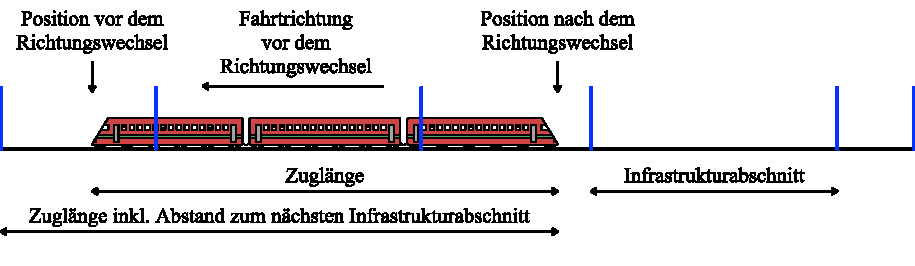
\includegraphics[width=\linewidth]{../images/vector/richtungsaenderung.pdf}
  \caption{Eigene Darstellung der Positionsbestimmung bei einem Richtungswechsel}
  \label{fig:richtungsaenderung}
\end{figure}
Damit die Richtungsänderung auch funktioniert, wenn das Fahrzeug nicht am Ende eines Infrastrukturabschnitts steht, wird für die Ermittlung der neuen Position auf die Fahrzeuglänge der Abstand bis zum Ende Infrastrukturabschnitts addiert (siehe Abbildung \ref{fig:richtungsaenderung}). Über den aktuellen und die folgenden Infrastrukturabschnitte (ermittelt durch die Funktion \textit{getNaechsteAbschnitte$($$)$}$^\ast$, des aktuellen Infrastrukturabschnitts und der neuen Richtung) wird iteriert und die Summe der Längen gebildet, bis die Fahrzeuglänge (zuzüglich des Abstands bis zum Ende des Infrastrukturabschnitts) überschritten wird. Der Infrastrukturabschnitt, in dem die Fahrzeuglänge inkl. des Abstands zum ersten Mal überschritten wird, entspricht dem Infrastrukturabschnitt der neuen Position.

Sollte die Länge aller nächsten Abschnitte inklusive des aktuellen Abschnitts in der Summe kleiner sein, als die Zuglänge inkl. dem Abstands bis zum Ende des Infrastrukturabschnitts, so kann die neue Position nicht ermittelt werden und dem Fahrzeug wird eine Fehlermeldung übergeben, sodass das Fahrzeug nicht weiter fahren wird. Andernfalls wird die Richtung des Fahrzeugs in der Datenbank geändert und dem Fahrzeug mit der Funktion \textit{sendFahrzeugbefehl$($$)$}$^\ast$ die Geschwindigkeit $-4km/h$ (entspricht einem Wendeauftrag) übergeben.

Bei einem Fahrtverlauf kann es vorkommen, dass Fahrzeuge mit Fahrplan auf der Fahrt mehrere Betriebsstellen passieren. Damit dem Eintrag \textit{angekommen} dieser Betriebsstellen auch der Wert \textit{true} zugewiesen werden kann, wird überprüft, ob in den \Gls{echtzeitdaten} dem Eintrag \textit{live\_all\_targets\_reached} ein Wert zugewiesen ist. Dieser Eintrag enthält - falls das Fahrzeug eine Betriebsstelle erreicht hat - den Index der Betriebsstelle und weist der Betriebsstelle unter dem Eintrag \textit{angekommen} den Wert \textit{true} zu.

Wenn die letzten \Gls{echtzeitdaten} eines Fahrzeugs übermittelt wurden (\textit{live\_target\_reached} == \textit{true}) und das Fahrzeug dementsprechend zum Stehen gekommen ist, wird überprüft, wie sich das Fahrzeug als nächstes verhalten soll. Dafür wird zwischen vier Fällen (siehe Tabelle \ref{table:vierfaelle}) unterschieden.
\begin{table}
\begin{center}
\renewcommand{\arraystretch}{1.2}
\begin{tabular}{c|c|c}
 & Fährt jetzt ohne Fahrplan & Fährt jetzt nach Fahrplan \\ \hline
Fuhrt davor ohne Fahrplan                 		&    1. Fall         & 2. Fall       \\ \hline
Fuhrt davor nach Fahrplan                   		&    3. Fall         & 4. Fall       \\ 
\end{tabular}
\renewcommand{\arraystretch}{1}
\caption{Verhalten eines Fahrzeugs nach dem Erreichen des Ziels}
\label{table:vierfaelle}
\end{center}
\end{table}
Für die Überprüfung, ob sich der Fahrplan eines Fahrzeugs geändert hat, wird über die Funktion \textit{getFahrzeugZugIds$($$)$} die aktuelle Zug-ID abgefragt und mit der vorherigen verglichen. In dem \textbf{1. Fall} (alte und neue Zug-ID haben beide den Wert \textit{null}) werden dem Fahrzeug keine neue Daten übergeben und ein neuer Fahrtverlauf wird versucht zu berechnen, sobald die Fahrstraße sich verändert hat. In dem \textbf{2.} und \textbf{4. Fall} wird die neue Zug-ID dem Fahrzeug übergeben, der Eintrag \textit{operates\_on\_timetable} auf \textit{true} gesetzt und die Funktionen \textit{getFahrplanAndPositionForOneTrain$($$)$}, \textit{addStopsectionsForTimetable$($$)$}, \textit{calculateNextSections$($$)$}, \textit{checkIfFahrstrasseIsCorrrect$($$)$} und \textit{calculateFahrverlauf$($$)$} aufgerufen. Abgesehen von der ersten Funktion, werden diese Funktionen auch beim Start des Programms ausgeführt, welcher in Kapitel \ref{main_2} beschrieben wird. Die Funktion \textit{get\-Fahrplan\-And\-Position\-For\-One\-Train$($$)$} ähnelt der in Kapitel \ref{main_2} beschrieben Funktion \textit{prepareTrainForRide$($$)$}, fügt aber nur die Position und den Fahrplan hinzu, da alle anderen Daten schon eingelesen wurden. In dem \textbf{3. Fall} (die neu ermittelte Zug-ID hat den Wert \textit{null}) wird der Eintrag \textit{operates\_on\_timetable} auf \textit{false} gesetzt und die Funktionen \textit{calculateNextSections$($$)$} und \textit{calculateFahrverlauf$($$)$} aufgerufen.
\subsection{Überprüfung nach einer Änderung der Fahrstraße}
Für die Überprüfung, ob sich die Fahrstraße der Züge verändert hat, wird in regelmäßigen Abständen die Fahrstraße der Fahrzeuge ermittelt und mit der aktuell hinterlegten Fahrstraße verglichen. Das Intervall, in dem diese Überprüfung stattfindet kann über die Variable \textit{\$timeCheckFahrstrasseInterval} (\textit{main.php}) festgelegt werden und ist standardgemäß auf 3 Sekunden festgelegt. Bei der Ermittlung und dem Vergleich der Fahrstraße wird für jedes Fahrzeug die Funktion \textit{compareTwoNaechsteAbschnitte$($$)$} aufgerufen. Innerhalb dieser Funktion wird die in Kapitel \ref{main_2} erläutere Funktion \textit{calculateNextSections$($$)$} aufgerufen, mit dem Unterschied, dass die ermittelten nächsten Infrastrukturabschnitte inkl. der Längen und zulässigen Höchstgeschwindigkeiten nicht dem Fahrzeug hinterlegt werden, sondern lokal in der Funktion gespeichert. Damit die ermittelten Daten für ein Fahrzeug berechnet werden, aber nicht dem Fahrzeug hinterlegt werden, kann der Parameter \textit{\$writeResultToTrain} der Funktion \textit{calculateNextSections$($$)$} (standardgemäß auf \textit{true} gesetzt) auf \textit{false} gesetzt werden.
\subsection{Neukalibrierung der Fahrzeugposition}  \label{main_5}
Für eine genau Fahrzeugsteuerung ist die aktuelle Position der Züge \textbf{essenziäl!} und muss während der Fahrt kalibriert werden, damit Ungenauigkeiten ausgeglichen werden können. Dafür werden die Daten aus der \textit{SQL}-Tabelle \textit{fahrzeuge\_abschnitte} benötigt, welche durch Abschnittsüberwachung ermittelt werden. Die Abschnittsüberwachung schreibt für jedes Fahrzeug den aktuellen Infrastrukturabschnitt in die Datenbank, sobald der Zugkopf den Abschnitt befährt inklusive der aktuellen Zeit (Realzeit). Für jedes Fahrzeug, welches durch die Übermittlung der \Gls{echtzeitdaten} in einen neuen Infrastrukturabschnitt einfährt und seit der Einfahrt in den Abschnitt die Geschwindigkeit nicht verändert hat, wird die aktuelle Position neu ermittelt. Würde sich das Fahrzeug in einem Abschnitt befinden und hätte seit der Einfahrt die Geschwindigkeit angepasst, könnte mit der Fahrzeugsteuerung die Position nicht neu berechnet werden, da nicht bekannt ist, welche Strecke das Fahrzeug seit der Einfahrt zurückgelegt. Aus diesem Grund wird, sobald das Fahrzeug laut den \Gls{echtzeitdaten} einen neuen Abschnitt befährt und aktuell nicht die Geschwindigkeit anpasst (\textit{live\_is\_speed\_change} == \textit{false}), dem Eintrag \textit{calibrate\_section\_one} der aktuelle Infrastrukturabschnitt hinzugefügt und dem Eintrag \textit{calibrate\_section\_two} wird ebenfalls der aktuelle Infrastrukturabschnitt hinzugefügt, wenn \textit{calibrate\_section\_one} ein Wert zugewiesen ist und dieser nicht dem aktuellen Infrastrukturabschnitt der \Gls{echtzeitdaten} entspricht. Soabld das Fahrzeug seine Geschwindigkeit anpasst (\textit{live\_is\_speed\_change} == \textit{true}), wird beiden Einträgen der Wert \textit{null} zugewiesen. Dadurch ist dem Eintrag \textit{calibrate\_section\_two} nur dann ein Infrastrukturabschnitt zugewiesen, wenn das Fahrzeug in diesem seit der Einfahrt die Geschwindigkeit nicht verändert hat. Wenn dem Eintrag \textit{\$useRecalibration} aus der Datei \textit{globalVariables.php} der Wert \textit{true} zugewiesen ist, wird in regelmäßigen Abständen überprüft, ob eine Neukalibrierung möglich ist. Das Zeitintervall, in dem die Überprüfung stattfindet ist standardmäßig auf auf 3 Sekunden eingestellt, kann aber mittels der Variable \textit{\$timeCheckCalibrationInterval} (\textit{main.php}) angepasst werden.

Für die Neukalibrierung wird die Funktion \textit{getCalibratedPosition$($$)$} (Code-Beispiel \ref{lst:getCalibratedPosition}) aufgerufen, welche als Rückgabewert die aktuelle relative Position und den aktuellen Infrastrukturabschnitt zurückgibt.
\begin{figure}
\begin{lstlisting}[caption={\textit{getCalibratedPosition$($$)$} (main.php)},captionpos=b,label={lst:getCalibratedPosition}]
function getCalibratedPosition ($id, $speed) {
	global $cacheFahrzeugeAbschnitte;
	$DB = new DB_MySQL();
	$positionReturn = $DB->select("SELECT `".DB_TABLE_FAHRZEUGE_ABSCHNITTE."`.`infra_id`, `".DB_TABLE_FAHRZEUGE_ABSCHNITTE."`.`unixtimestamp` FROM `".DB_TABLE_FAHRZEUGE_ABSCHNITTE."` WHERE `".DB_TABLE_FAHRZEUGE_ABSCHNITTE."`.`fahrzeug_id` = $id")[0];
	unset($DB);
	if (in_array($id, array_keys($cacheFahrzeugeAbschnitte))) {
		if ($positionReturn->unixtimestamp == $cacheFahrzeugeAbschnitte[$id]["unixtimestamp"]) {
			return array("possible" => false);
		}
	}
	$timeDiff = time() - $positionReturn->unixtimestamp;
	$position = ($speed / 3.6) * $timeDiff;
	return array("possible" => true, "section" => $positionReturn->infra_id, "position" => $position);
}
\end{lstlisting}
\end{figure}
Sollte die ermittelte Position innerhalb des Abschnitts größer als die Länge des Abschnitts, welche in dem Array \textit{\$cacheInfraLaenge} abgespeichert ist, sein, wird die Neukalibrierung nicht durchgeführt. Der aktuelle Infrastrukturabschnitt wird aus der Tabelle \textit{fahrzeuge\_abschnitte} der Datenbank geladen und durch die aktuelle Geschwindigkeit des Fahrzeugs und die Differenz der Zeit zwischen dem Einfahren in den Abschnitt und der aktuellen Zeit wird die relative Position innerhalb des Abschnitts berechnet.
\begin{figure}
\[\textrm{relative Position} = \textrm{Geschwindigkeit} \cdot \textrm{Zeitdifferenz (aktuelle Zeit} - \textrm{Zeit des Einfahrens)}\]
\end{figure}
\subsection{Ermittlung von neuen Fahrzeugen im eingleisigen Netz} \label{main_6}
Die Fahrzeugsteuerung betrachtet neben den Fahrzeugen, welche sich schon zu Beginn des Programmstarts im eingleisigen Netz befinden auch alle Fahrzeuge, die nach dem Programmstart hinzugefügt werden. Für alle Fahrzeuge, die beim Start des Programms erkannt werden, wird in dem Array \textit{\$allTrainsOnTheTrack} die zugehörige Adresse gespeichert (\textit{find\-Trains\-On\-The\-Tracks$($$)$}). Für die Überprüfung, ob Fahrzeuge entfernt wurden oder neu hinzugekommen sind, wird die Funktion \textit{updateAllTrainsOnTheTrack$($$)$} verwendet. Diese Funktion wird - wie die Neukalibrierung in Kapitel \ref{main_5} - alle 3 Sekunden ausgeführt. Bei dem Aufruf der Funktion werden alle Fahrzeuge geladen, denen in der \textit{fma}-Tabelle aus der Datenbank ein Infrastrukturabschnitt zugeordnet ist und mit dem Array \textit{\$allTrainsOnTheTrack} verglichen. Fahrzeugadressen, die nicht in dem Array hinterlegt sind, werden in dem Rückgabe-Array unter dem Eintrag \textit{new} zurückgegeben und alle Fahrzeugadressen, die in dem Array enthalten sind, aber bei dem Aufruf der Funktion keinem Infrastrukturabshcnitt zugeordnet sind, werden in dem Rückgabe-Array unter dem Eintrag \textit{removed} zurückgegeben. Nach dem Aufruf der Funktion, werden für alle neuen Fahrzeuge die Funktion \textit{prepare\-Train\-For\-Ride$($$)$}, \textit{add\-Stopsections\-For\-Timetable$($$)$}, \textit{calculate\-Next\-Sections$($$)$}, \textit{check\-If\-Train\-Reached\-Haltepunkt$($$)$}, \textit{check\-If\-Fahrstrasse\-Is\-Corrrect$($$)$} und \textit{calculate\-Fahrverlauf$($$)$} aufgerufen (siehe Kapitel \ref{main_2} und \ref{main_3}). Alle entfernten Fahrzeuge werden aus dem Array \textit{\$allUsedTrains} entfernt und somit nicht mehr von der Fahrzeugsteuerung beachtet. 







































